%  A simple AAU report template.
%  2015-05-08 v. 1.2.0
%  Copyright 2010-2015 by Jesper Kjær Nielsen <jkn@es.aau.dk>
%
%  This is free software: you can redistribute it and/or modify
%  it under the terms of the GNU General Public License as published by
%  the Free Software Foundation, either version 3 of the License, or
%  (at your option) any later version.
%
%  This is distributed in the hope that it will be useful,
%  but WITHOUT ANY WARRANTY; without even the implied warranty of
%  MERCHANTABILITY or FITNESS FOR A PARTICULAR PURPOSE.  See the
%  GNU General Public License for more details.
%
%  You can find the GNU General Public License at <http://www.gnu.org/licenses/>.
%
%  A simple AAU report template.
%  2015-05-08 v. 1.2.0
%  Copyright 2010-2015 by Jesper Kjær Nielsen <jkn@es.aau.dk>
%
%  This is free software: you can redistribute it and/or modify
%  it under the terms of the GNU General Public License as published by
%  the Free Software Foundation, either version 3 of the License, or
%  (at your option) any later version.
%
%  This is distributed in the hope that it will be useful,
%  but WITHOUT ANY WARRANTY; without even the implied warranty of
%  MERCHANTABILITY or FITNESS FOR A PARTICULAR PURPOSE.  See the
%  GNU General Public License for more details.
%
%  You can find the GNU General Public License at <http://www.gnu.org/licenses/>.
%
\documentclass[11pt,twoside,a4paper,openright]{report}
%%%%%%%%%%%%%%%%%%%%%%%%%%%%%%%%%%%%%%%%%%%%%%%%
% Language, Encoding and Fonts
% http://en.wikibooks.org/wiki/LaTeX/Internationalization
%%%%%%%%%%%%%%%%%%%%%%%%%%%%%%%%%%%%%%%%%%%%%%%%
% Select encoding of your inputs. Depends on
% your operating system and its default input
% encoding. Typically, you should use
%   Linux  : utf8 (most modern Linux distributions)
%            latin1 
%   Windows: ansinew
%            latin1 (works in most cases)
%   Mac    : applemac
% Notice that you can manually change the input
% encoding of your files by selecting "save as"
% an select the desired input encoding. 
\usepackage[utf8]{inputenc}
% Make latex understand and use the typographic
% rules of the language used in the document.
\usepackage[,english]{babel}
% Use the palatino font
\usepackage[sc]{mathpazo}
\usepackage[numbered,framed]{matlab-prettifier}
\linespread{1.05}         % Palatino needs more leading (space between lines)
% Choose the font encoding
\usepackage[T1]{fontenc}
%%%%%%%%%%%%%%%%%%%%%%%%%%%%%%%%%%%%%%%%%%%%%%%%
% Graphics and Tables
% http://en.wikibooks.org/wiki/LaTeX/Importing_Graphics
% http://en.wikibooks.org/wiki/LaTeX/Tables
% http://en.wikibooks.org/wiki/LaTeX/Colors
%%%%%%%%%%%%%%%%%%%%%%%%%%%%%%%%%%%%%%%%%%%%%%%%
% load a colour package
\usepackage{xcolor}
\definecolor{aaublue}{RGB}{33,26,82}% dark blue
% The standard graphics inclusion package
\usepackage{graphicx}
% Set up how figure and table captions are displayed
\usepackage{caption}
\captionsetup{%
  font=footnotesize,% set font size to footnotesize
  labelfont=bf % bold label (e.g., Figure 3.2) font
}
% Make the standard latex tables look so much better
\usepackage{array,booktabs}
% Enable the use of frames around, e.g., theorems
% The framed package is used in the example environment
\usepackage{framed}

%%%%%%%%%%%%%%%%%%%%%%%%%%%%%%%%%%%%%%%%%%%%%%%%
% Mathematics
% http://en.wikibooks.org/wiki/LaTeX/Mathematics
%%%%%%%%%%%%%%%%%%%%%%%%%%%%%%%%%%%%%%%%%%%%%%%%
% Defines new environments such as equation,
% align and split 
\usepackage{amsmath}
% Adds new math symbols
\usepackage{amssymb}
% Use theorems in your document
% The ntheorem package is also used for the example environment
% When using thmmarks, amsmath must be an option as well. Otherwise \eqref doesn't work anymore.
\usepackage[framed,amsmath,thmmarks]{ntheorem}

%%%%%%%%%%%%%%%%%%%%%%%%%%%%%%%%%%%%%%%%%%%%%%%%
% Page Layout
% http://en.wikibooks.org/wiki/LaTeX/Page_Layout
%%%%%%%%%%%%%%%%%%%%%%%%%%%%%%%%%%%%%%%%%%%%%%%%
% Change margins, papersize, etc of the document
\usepackage[
  inner=28mm,% left margin on an odd page
  outer=41mm,% right margin on an odd page
  ]{geometry}
% Modify how \chapter, \section, etc. look
% The titlesec package is very configureable
\usepackage{titlesec}
\titleformat{\chapter}[display]{\normalfont\huge\bfseries}{\chaptertitlename\ \thechapter}{20pt}{\Huge}
\titleformat*{\section}{\normalfont\Large\bfseries}
\titleformat*{\subsection}{\normalfont\large\bfseries}
\titleformat*{\subsubsection}{\normalfont\normalsize\bfseries}
%\titleformat*{\paragraph}{\normalfont\normalsize\bfseries}
%\titleformat*{\subparagraph}{\normalfont\normalsize\bfseries}

% Clear empty pages between chapters
\let\origdoublepage\cleardoublepage
\newcommand{\clearemptydoublepage}{%
  \clearpage
  {\pagestyle{empty}\origdoublepage}%
}
\let\cleardoublepage\clearemptydoublepage

% Change the headers and footers
\usepackage{fancyhdr}
\pagestyle{fancy}
\fancyhf{} %delete everything
\renewcommand{\headrulewidth}{0pt} %remove the horizontal line in the header
\fancyhead[RE]{\small\nouppercase\leftmark} %even page - chapter title
\fancyhead[LO]{\small\nouppercase\rightmark} %uneven page - section title
\fancyhead[LE,RO]{\thepage} %page number on all pages
% Do not stretch the content of a page. Instead,
% insert white space at the bottom of the page
\raggedbottom
% Enable arithmetics with length. Useful when
% typesetting the layout.
\usepackage{calc}

%%%%%%%%%%%%%%%%%%%%%%%%%%%%%%%%%%%%%%%%%%%%%%%%
% Bibliography
% http://en.wikibooks.org/wiki/LaTeX/Bibliography_Management
%%%%%%%%%%%%%%%%%%%%%%%%%%%%%%%%%%%%%%%%%%%%%%%%
\usepackage{csquotes}
\usepackage[backend=bibtex, bibencoding=utf8, sorting=nty]{biblatex}
\addbibresource{bib/mybib}

%%%%%%%%%%%%%%%%%%%%%%%%%%%%%%%%%%%%%%%%%%%%%%%%
% Misc
%%%%%%%%%%%%%%%%%%%%%%%%%%%%%%%%%%%%%%%%%%%%%%%%
% Add bibliography and index to the table of
% contents
\usepackage[nottoc]{tocbibind}
% Add the command \pageref{LastPage} which refers to the
% page number of the last page
\usepackage{lastpage}
% Add todo notes in the margin of the document
\usepackage[
%  disable, %turn off todonotes
  colorinlistoftodos, %enable a coloured square in the list of todos
  textwidth=\marginparwidth, %set the width of the todonotes
  textsize=scriptsize, %size of the text in the todonotes
  ]{todonotes}

%%%%%%%%%%%%%%%%%%%%%%%%%%%%%%%%%%%%%%%%%%%%%%%%
% Hyperlinks
% http://en.wikibooks.org/wiki/LaTeX/Hyperlinks
%%%%%%%%%%%%%%%%%%%%%%%%%%%%%%%%%%%%%%%%%%%%%%%%
% Enable hyperlinks and insert info into the pdf
% file. Hypperref should be loaded as one of the 
% last packages
\usepackage{hyperref}
\hypersetup{%
	pdfpagelabels=true,%
	plainpages=false,%
	pdfauthor={Author(s)},%
	pdftitle={Title},%
	pdfsubject={Subject},%
	bookmarksnumbered=true,%
	colorlinks=false,%
	citecolor=black,%
	filecolor=black,%
	linkcolor=black,% you should probably change this to black before printing
	urlcolor=black,%
	pdfstartview=FitH%
}% package inclusion and set up of the document
% see, e.g., http://en.wikibooks.org/wiki/LaTeX/Formatting#Hyphenation
% for more information on word hyphenation
\hyphenation{ex-am-ple hy-phen-a-tion short}
\hyphenation{long la-tex}% 
%  A simple AAU report template.
%  2015-05-08 v. 1.2.0
%  Copyright 2010-2015 by Jesper Kjær Nielsen <jkn@es.aau.dk>
%
%  This is free software: you can redistribute it and/or modify
%  it under the terms of the GNU General Public License as published by
%  the Free Software Foundation, either version 3 of the License, or
%  (at your option) any later version.
%
%  This is distributed in the hope that it will be useful,
%  but WITHOUT ANY WARRANTY; without even the implied warranty of
%  MERCHANTABILITY or FITNESS FOR A PARTICULAR PURPOSE.  See the
%  GNU General Public License for more details.
%
%  You can find the GNU General Public License at <http://www.gnu.org/licenses/>.
%
%
%
% see, e.g., http://en.wikibooks.org/wiki/LaTeX/Customizing_LaTeX#New_commands
% for more information on how to create macros

%%%%%%%%%%%%%%%%%%%%%%%%%%%%%%%%%%%%%%%%%%%%%%%%
% Macros for the titlepage
%%%%%%%%%%%%%%%%%%%%%%%%%%%%%%%%%%%%%%%%%%%%%%%%
%Creates the aau titlepage
\newcommand{\aautitlepage}[3]{%
  {
    %set up various length
    \ifx\titlepageleftcolumnwidth\undefined
      \newlength{\titlepageleftcolumnwidth}
      \newlength{\titlepagerightcolumnwidth}
    \fi
    \setlength{\titlepageleftcolumnwidth}{0.5\textwidth-\tabcolsep}
    \setlength{\titlepagerightcolumnwidth}{\textwidth-2\tabcolsep-\titlepageleftcolumnwidth}
    %create title page
    \thispagestyle{empty}
    \noindent%
    \begin{tabular}{@{}ll@{}}
      \parbox{\titlepageleftcolumnwidth}{
        \iflanguage{danish}{%
          \includegraphics[width=\titlepageleftcolumnwidth]{figures/aau_logo_da}
        }{%
          \includegraphics[width=\titlepageleftcolumnwidth]{figures/aau_logo_en}
        }
      } &
      \parbox{\titlepagerightcolumnwidth}{\raggedleft\sf\small
        #2
      }\bigskip\\
       #1 &
      \parbox[t]{\titlepagerightcolumnwidth}{%
      \textbf{Abstract:}\bigskip\par
        \fbox{\parbox{\titlepagerightcolumnwidth-2\fboxsep-2\fboxrule}{%
          #3
        }}
      }\\
    \end{tabular}
    \vfill
    \iflanguage{danish}{%
      \noindent{\footnotesize\emph{Rapportens indhold er frit tilgængeligt, men offentliggørelse (med kildeangivelse) må kun ske efter aftale med forfatterne.}}
    }{%
      \noindent{\footnotesize\emph{The content of this report is freely available, but publication (with reference) may only be pursued due to agreement with the author.}}
    }
    \clearpage
  }
}

%Create english project info
\newcommand{\englishprojectinfo}[8]{%
  \parbox[t]{\titlepageleftcolumnwidth}{
    \textbf{Title:}\\ #1\bigskip\par
    \textbf{Theme:}\\ #2\bigskip\par
    \textbf{Project Period:}\\ #3\bigskip\par
    \textbf{Project Group:}\\ #4\bigskip\par
    \textbf{Participant(s):}\\ #5\bigskip\par
    \textbf{Supervisor(s):}\\ #6\bigskip\par
    \textbf{Copies:} #7\bigskip\par
    \textbf{Page Numbers:} \pageref{LastPage}\bigskip\par
    \textbf{Date of Completion:}\\ #8
  }
}

%Create danish project info
\newcommand{\danishprojectinfo}[8]{%
  \parbox[t]{\titlepageleftcolumnwidth}{
    \textbf{Titel:}\\ #1\bigskip\par
    \textbf{Tema:}\\ #2\bigskip\par
    \textbf{Projektperiode:}\\ #3\bigskip\par
    \textbf{Projektgruppe:}\\ #4\bigskip\par
    \textbf{Deltager(e):}\\ #5\bigskip\par
    \textbf{Vejleder(e):}\\ #6\bigskip\par
    \textbf{Oplagstal:} #7\bigskip\par
    \textbf{Sidetal:} \pageref{LastPage}\bigskip\par
    \textbf{Afleveringsdato:}\\ #8
  }
}

%%%%%%%%%%%%%%%%%%%%%%%%%%%%%%%%%%%%%%%%%%%%%%%%
% An example environment
%%%%%%%%%%%%%%%%%%%%%%%%%%%%%%%%%%%%%%%%%%%%%%%%
\theoremheaderfont{\normalfont\bfseries}
\theorembodyfont{\normalfont}
\theoremstyle{break}
\def\theoremframecommand{{\color{gray!50}\vrule width 5pt \hspace{5pt}}}
\newshadedtheorem{exa}{Example}[chapter]
\newenvironment{example}[1]{%
		\begin{exa}[#1]
}{%
		\end{exa}
}% my new macros

\begin{document}
%frontmatter
%\pagestyle{empty} %disable headers and footers
%\pagenumbering{roman} %use roman page numbering in the frontmatter

%  A simple AAU report template.
%  2015-05-08 v. 1.2.0
%  Copyright 2010-2015 by Jesper Kjær Nielsen <jkn@es.aau.dk>
%
%  This is free software: you can redistribute it and/or modify
%  it under the terms of the GNU General Public License as published by
%  the Free Software Foundation, either version 3 of the License, or
%  (at your option) any later version.
%
%  This is distributed in the hope that it will be useful,
%  but WITHOUT ANY WARRANTY; without even the implied warranty of
%  MERCHANTABILITY or FITNESS FOR A PARTICULAR PURPOSE.  See the
%  GNU General Public License for more details.
%
%  You can find the GNU General Public License at <http://www.gnu.org/licenses/>.
%
\pdfbookmark[0]{Front page}{label:frontpage}%
\begin{titlepage}
  \addtolength{\hoffset}{0.5\evensidemargin-0.5\oddsidemargin} %set equal margins on the frontpage - remove this line if you want default margins
  \noindent%
  \begin{tabular}{@{}p{\textwidth}@{}}
    \toprule[2pt]
    \midrule
    \vspace{0.2cm}
    \begin{center}
    \Huge{\textbf{
      Applying laplacian smoothing on joint optimization problem
    }}
    \end{center}
    \vspace{0.2cm}\\
    \midrule
    \toprule[2pt]
  \end{tabular}
  \vspace{4 cm}
  \begin{center}
    {\Large
      Photorealistic Rendering%Insert document type (e.g., Project Report)
    }\\
    \vspace{0.4cm}
    {\Large
      Hyeonjang An\\[0.4cm]
      20211046 \\

    }
  \end{center}
  \vfill
  \begin{center}
    School of Integrated Technology \\
    GIST \\
    Autumn 2021
  \end{center}
\end{titlepage}
%\newpage
%\clearpage
%\input{sections/colophon.tex}
%\input{sections/titlepages.tex}
%\cleardoublepage
\pdfbookmark[0]{Contents}{label:contents}
\pagestyle{fancy} %enable headers and footers again
%\tableofcontents
%\listoftodos
\section*{Project Description}\label{ch:ch1label}

We would like to focus on a popular macroeconomics problem called Utility Maximization, where the goal is to maximize the happiness of a consumer. The utility function will be denoted by $ U(c,l) $, which relates the consumption and the leisure of an individual in society with his/her happiness. A simple utility function is log-sum of consumption and leisure. Often, a discount factor $\beta$ (a modeling constant) is applied exponentially. Discount factor is used to model gradually decreased effects of future wealth on today \cite{Macroeconomics}.

The function takes two arguments: $ c \in \mathbb{R}^n = (c_1,c_2,...,c_n)$ and $ l \in \mathbb{R}^n = (l_1,l_2,...,l_n) $ which denote the normalized $(c_t,l_t \in [0,1])$ consumption and labor. The price for the single consumption good is denoted as $ P = (P_1,P_2,...,P_n)  $. The consumer, at time step t, needs to prepare $m_t = P_tc_t$ amount of money for the next time step, $t+1$, which is called the cash-in-advance constraint. There is the bonds mechanism, on time step t, when a consumer buys bonds worth $s_t$, at next time step he/she receives $(1+R)s_t$ with R being the interest rate. The same applies while borrowing. The consumption and work hours spent (labor) is related with a production function, which is in general a concave function such as $ln(l_t)$ or $l_t^\alpha$ with $0 \leq \alpha \leq 1$ being a constant. To keep things simple, we have assumed R is not fluctuating.

To simplify the problem, there is a bold assumption of "representative household" and we can employ that. This basically means that rather than modeling and optimizing for a single household, it is possible to optimize for a "representative" which is an arithmetic mean of the entire population. This approach introduces two more constraints, known as market-clearing constraints: $ s_t = 0 $ since on average, no-one can borrow without a lender and 
$ c_t = f(l_t)  $ since on average, a good which is not produced cannot be consumed. \\
\\The formal (mathematical) statement of our problem is:
\begin{equation*}
\begin{aligned}
& \underset{ \{ c_t,l_t,s_{t+1},m_{t+1} \} }{\text{maximize}}
& & U(c,l) = \sum_{t=0}^{N-}{\beta^t}[ln(c_t)+ln(1-l_t)] \\
& \text{subject to}
& & P_tc_t=m_t\\
& & & m_{t+1}+s_{t+1}=m_t+(1+R_t)s_t+P_tl_t+\tau_t-P_tc_t \\
& & & c_t = l_t \quad \text{to see effects of production function to optimization problem} \\
& & & s_t = 0
\end{aligned}
\end{equation*}
The formal version of problem is generally not solved numerically, instead it is solved algebraically and then expressions for terms are found and comments are made on them. However, in this project, after those steps, we would like to carry the problem to the numeric "domain" and visually see how environment parameters affect consumer decisions. In order to be able to solve with MATLAB, we need to add 2 more constraints, to bound c and l (normalize them). These constraints are:
\begin{align*}
0 \preceq c \preceq 1 \textrm{ and } 0 \preceq l \preceq 1
\end{align*}
These will not be derived in duality \& kkt sections however their effects will be expressed within simulation section.

%\cleardoublepage
%mainmatter
\pagenumbering{arabic} %use arabic page numbering in the mainmatter
%\chapter{Introduction}\label{ch:introduction}
Here is the introduction. The next chapter is chapter~\ref{ch:ch2label}.


a new paragraph


\section{Examples}
You can also have examples in your document such as in example~\ref{ex:simple_example}.
\begin{example}{An Example of an Example}
  \label{ex:simple_example}
  Here is an example with some math
  \begin{equation}
    0 = \exp(i\pi)+1\ .
  \end{equation}
  You can adjust the colour and the line width in the {\tt macros.tex} file.
\end{example}

\section{How Does Sections, Subsections, and Subsections Look?}
Well, like this
\subsection{This is a Subsection}
and this
\subsubsection{This is a Subsubsection}
and this.

\paragraph{A Paragraph}
You can also use paragraph titles which look like this.

\subparagraph{A Subparagraph} Moreover, you can also use subparagraph titles which look like this\todo{Is it possible to add a subsubparagraph?}. They have a small indentation as opposed to the paragraph titles.

\todo[inline,color=green]{I think that a summary of this exciting chapter should be added.}
\section*{Discussion of Convexity}\label{ch:ch2label}
We discuss the convexity of the objective function by observing that $U(c,l)$ is a weighted sum of functions depending on $c_{t}, l_{t}$.
\\
\begin{equation*}
\implies U(c,l) = \sum_{t=0}^{N-1}{\beta^{t}}[f(c_t,l_t)]
\end{equation*}
Let us consider $\beta^t, c_t, f(c_t, l_t)$ and $l_t$ as vectors of length N. $\rightarrow$ $\beta, c, f(c, l), l$.
\begin{equation*}
\implies U(c,l) = \beta^T[f(c,l)]
\end{equation*}
We see that $U(c,l)$ is an affine function of $f(c,l)$, and that $\beta \succeq 0$. Therefore, for the optimization problem to be convex, we need to analyze the concavity of $f(c,l)$. In this case, because of the affine combination property, it is sufficient to check if $f(c_t,l_t)$ is concave. We look at the Hessian of $f(c_t,l_t)$.\\

\begin{minipage}{0.4\textwidth}
\begin{align*}
\frac{\partial f}{\partial c_t} = \frac{1}{c_t} \implies \frac{\partial^2 f}{\partial c_t^2}= -\frac{1}{c_t^2}
\end{align*}
\end{minipage}
\begin{minipage}{0.6\textwidth}
\begin{align*}
\frac{\partial f}{\partial l_t}= -\frac{1}{1-l_t} \implies \frac{\partial^2 f}{\partial l_t^2}= -\frac{1}{(1-l_t)^2}
\end{align*}
\end{minipage}
\\
\begin{minipage}{0.5\textwidth}
\begin{align*}
\frac{\partial^2 f}{\partial c_t \partial l_t}= 0
\end{align*}
\end{minipage}
\begin{minipage}{0.5\textwidth}
\begin{align*}
\bigtriangledown^2f(c_t,l_t)= \begin{bmatrix}
-\frac{1}{c_t^2} & 0 \\
0 & -\frac{1}{(1-l_t)^2}
\end{bmatrix}
\preceq 0
\end{align*}
\end{minipage}
\\\\
The Hessian is a negative matrix, and therefore $f(c_t,l_t)$ is concave. Since each added term in the sum is concave, we conclude that the objective is a concave function.\\
\\For the constraints, we analyze the market-clearing conditions introduced in the previous section.\\
\begin{minipage}{0.15\textwidth}
\begin{align*}
s_{t+1}=s_{t}=0
\end{align*}
\end{minipage}
\begin{minipage}{0.15\textwidth}
\begin{align*}
c_{t}=l_{t}
\end{align*}
\end{minipage}
\begin{minipage}{0.15\textwidth}
\begin{align*}
P_t c_{t}=m_{t}
\end{align*}
\end{minipage}
\begin{minipage}{0.55\textwidth}
\begin{align*}
\implies m_{t+1}=m_t+\tau_t=m_t+gm_t=m_t(1+g)
\end{align*}
\end{minipage}
\\
\\All constraints are linear and thus convex; therefore we can solve the problem using convex optimization techniques.






\section*{Formulation of the Dual Problem - Part 1}\label{ch:ch3label}
We write the Lagrangian with the dual variables $\beta^t \mu_t$, $\beta^t \lambda_t$, $\beta^ty_t$ and $\beta^t z_t$:

\begin{align*}
L(c_t,l_t,s_{t+1},m_{t+1},\mu_{t},\lambda_t,y_t,z_t) &= \sum_{t=0}^{N-1}{\beta^t}[\ln(c_t)+\ln(1-l_t)+\mu_t(m_t- P_t c_t)]\\
&\quad+\sum_{t=0}^{N-2}{\beta^t}\lambda_t(m_t+(1+R_t)s_t+P_t l_t + \tau_t - P_t c_t - m_{t+1} - s_{t+1})\\
&\quad+\sum_{t=0}^{N-1}{\beta^t}(y_t(c_t-l_t)+z_t(s_t))
\end{align*}
In order to find the dual, we note that as two constraints, we will need $y_t=0$ and $z_t = 0$ otherwise the supremum would tend to infinity. Therefore,
\begin{align*}
g(\lambda_t,\mu_t) = \sup_{c_t,l_t,s_{t+1},m_{t+1}}L
\end{align*} we set the gradient of the Lagrangian to zero since the Lagrangian is concave. This brings us to the KKT conditions, but we will return to this discussion.
\section*{KKT Conditions}\label{ch:ch4label}
In order to obtain the KKT conditions, we set the gradient of the Lagrangian to zero. $\bigtriangledown L = 0$. We do not have any inequality constraints, so we will not look at complementary slackness. Instead of using the dual variable $y_t$ for the constraint $c_t=l_t$, we will simplify the problem by replacing $l_t$ with $c_t$.
\begin{align}{\label{eq1}}
	\frac{dL}{dc_t} = 0 \implies \beta^t\frac{1}{c_t}-\beta^t(\mu_t+\lambda_t)P_t=0 \implies \frac{1}{c_t}=(\mu_t+\lambda_t)P_t
\end{align}
\begin{align}{\label{eq2}}
	\frac{dL}{dl_t} = 0 \implies -\beta^t\frac{1}{1-l_t}+\beta^t\lambda_t P_t=0 \implies \lambda_t = \frac{1}{(1-l_t)P_t}
\end{align}
\begin{align}{\label{eq3}}
	\frac{dL}{ds_{t+1}} = 0 \implies -\beta^t\lambda_t+\beta^{t+1}\lambda_{t+1}(1+R_{t+1})=0 \implies \lambda_t = \beta \lambda_{t+1}(1+R_{t+1})
\end{align}
\begin{align}{\label{eq4}}
	\frac{dL}{dm_{t+1}} = 0 \implies -\beta^t\lambda_t+\beta^{t+1}(\mu_{t+1}+\lambda_{t+1})=0 \implies \beta(\mu_{t+1}+\lambda_{t+1})=\lambda_t
\end{align}
Using equation (\ref{eq1}) and equation (\ref{eq4}), we get an expression for $\lambda$ and we plug this in equation (\ref{eq2}). We also use the constraint $c_t=l_t$.
\begin{align}{\label{eq5}}
	\lambda_t=\frac{\beta}{c_{t+1}P_{t+1}} = \frac{1}{(1-c_t)P_t} \implies \frac{P_{t+1}}{P_t} = \beta\frac{1-c_t}{c_t+1}
\end{align}
We also use equation (\ref{eq2}) in equation (\ref{eq3}).
\begin{align}{\label{eq6}}
	\frac{1}{(1-c_t)P_t}=\frac{\beta(1+R_{t+1})}{(1-c_{t+1})P_{t+1}} \implies \frac{P_{t+1}}{P_t}=\frac{1-c_t}{1-c_{t+1}}\beta(1+R_{t+1})
\end{align}
Finally, we have $P_t c_t = m_t$.
\begin{align}{\label{eq7}}
	\frac{P_{t+1}}{P_t}=\frac{(1+\tau_t/m_t)c_{t+1}}{c_t}=\frac{1-c_t}{1-c_{t+1}}\beta(1+R_{t+1})=\beta\frac{1-c_t}{c_{t+1}}
\end{align}
Using the equalities in (\ref{eq7}), we find that
\begin{align}{\label{eq8}}
	c_{t+1} = \frac{1}{2+R_{t+1}}
\end{align}
and all three equalities in (\ref{eq7}) are satisfied if $c_{t+1}=c_t \implies c_t =c^*$ is a constant; consequently, $R_t=R$ and $l_t = l^*$ are constants as well, and 
\begin{align}{\label{eq9}}
	1+\frac{\tau_t}{m_t} = \beta(1+R_t) \implies \frac{\tau_t}{m_t}=g \rightarrow \textrm{constant}
\end{align}
For optimal conditions, we set $l_t = c_t = c^*$ in $\sum_{t=0}^{N-1}{\beta^t}[ln(c_t)+ln(1-l_t)]$ and set its derivative to zero, since the objective is reduced to one variable.
\begin{align}{\label{eq10}}
	\frac{d}{dc^*}\frac{1-\beta^N}{1-\beta}[ln(c^*)+ln(1-c^*)]=0 \implies \frac{1}{c^*}-\frac{1}{1-c^*}=0 \implies c^* = 1/2
\end{align}
Since $c^*=\frac{1}{2+R} \implies R = 0$ and $g=\beta-1$. The optimal values are $m_{t+1}^*=\beta m_t \implies m_{t+1} = \beta^(t+1) m_0$, $s_{t+1}=0$, $c_{t} = l_{t} = 1/2$ for the system in equilibrium for N days.
\section*{Formulation of the Dual Problem - Part 2}\label{ch:ch3_2label}
We have\\
\begin{minipage}{0.2\textwidth}
\begin{align*}
	l_t = 1-\frac{1}{\lambda_t P_t}  
\end{align*}
\end{minipage}
\begin{minipage}{0.2\textwidth}
\begin{align*}
	 c_t = \frac{1}{(\mu_t+\lambda_t)P_t}
\end{align*}
\end{minipage}
\begin{minipage}{0.2\textwidth}
\begin{align*}
	s_{t+1} = 0
\end{align*}
\end{minipage}
\begin{minipage}{0.2\textwidth}
\begin{align*}
	m_{t+1} = m_t(1+\tau_t/m_t)=\frac{1+g}{(\mu_t+\lambda_t)}
\end{align*}
\end{minipage}
\\
\begin{minipage}{0.4\textwidth}
\begin{align*}
	\lambda_t = \beta \lambda_{t+1}(1+R_{t+1})
\end{align*}
\end{minipage}
\begin{minipage}{0.4\textwidth}
\begin{align*}
	\beta(\mu_{t+1}+\lambda_{t+1})=\lambda_t
\end{align*}
\end{minipage}
\begin{align*}
g(\lambda_t,\mu_t) &= \sum_{t=0}^{N-1}{\beta^t}[\ln(\frac{1}{(\mu_t+\lambda_t)P_t})+\ln(\frac{1}{\lambda_t P_t})+\mu_t(m_t-\frac{1}{(\mu_t+\lambda_t)} )]\\
&\quad+\sum_{t=0}^{N-2}{\beta^t}\lambda_t(m_t+(1+R_t)s_t+P_t(1-\frac{1}{\lambda_t}) + \tau_t - \frac{1}{(\mu_t+\lambda_t)} - \frac{1+g}{(\mu_t+\lambda_t)} )
\end{align*}
The dual problem then becomes
\begin{align*}
	\textrm{minimize} \quad\quad\quad\quad g(\lambda_t,\mu_t)
\end{align*}
\begin{align*}
	\textrm{subject to} \quad\quad\quad\quad s_t = 0
\end{align*}
\begin{align*}
	1-\frac{1}{\lambda_t P_t} = \frac{1}{(\mu_t+\lambda_t)P_t}
\end{align*}
\begin{align*}
	\lambda_t = \beta \lambda_{t+1}(1+R_{t+1})
\end{align*}
\begin{align*}
	\beta(\mu_{t+1}+\lambda_{t+1})=\lambda_t
\end{align*}
\section*{Simulation Results and Discussion}\label{ch:ch5label}

Let us first try only with cash-in-advance, money flow and normalizing (c and l being between 0 and 1) constraints. In this case, we are just trying to maximize for a single person. Let us also assume that the individual begins with a fair amount of money (0.5 units) so that he does not starve in the first time step.

The result: c = [1,1,...,1] and l = [0,0,...,0] regardless of the interest rate, prices, discount factor and any other variable. It is a bit weird that the consumer is able to consume a lot without actually working. What we notice is that amount of bond bought is [3.5,3,...] yet the debts are not paid. So a Ponzi scheme is created. The consumer borrows more and more each round. Even though not being an economically valid result, let us analyze in terms of convex optimization terminology. Currently, the only active constraints are normalizing constraints (i.e. $0 \leq c \leq 1$). So the Lagrange multipliers for those are strictly positive and the rest are zero.

Now let us try adding ponzi scheme preventing constraint in the last time step, s (amount of bonds) should be zero since the consumer will not be existent in next time step.

$s_{N-1} = 0$ 

In this case, R, $\beta$ and other modeling parameters begin to matter. Let us include a 3D graph of c(t) versus $\beta$.

\begin{figure}
\caption{Optimal consumption strategy for various $\beta$ and $m(1)=0.5$, R=0, no market clearing, Ponzi not allowed}
\centering
\includegraphics[width=12cm,height=8cm]{figures/r0_consumption.pdf}
\end{figure}


\begin{figure}
\caption{Optimal labor strategy for various $\beta$ and $m(1)=0.5$, R=0, no market clearing, Ponzi not allowed}
\centering
\includegraphics[width=12cm,height=8cm]{figures/r0_labor.pdf}
\end{figure}


\begin{figure}
\caption{Optimal consumption strategy for various $\beta$ and $m(1)=0.5$, R=0.8, no market clearing, Ponzi not allowed}
\centering
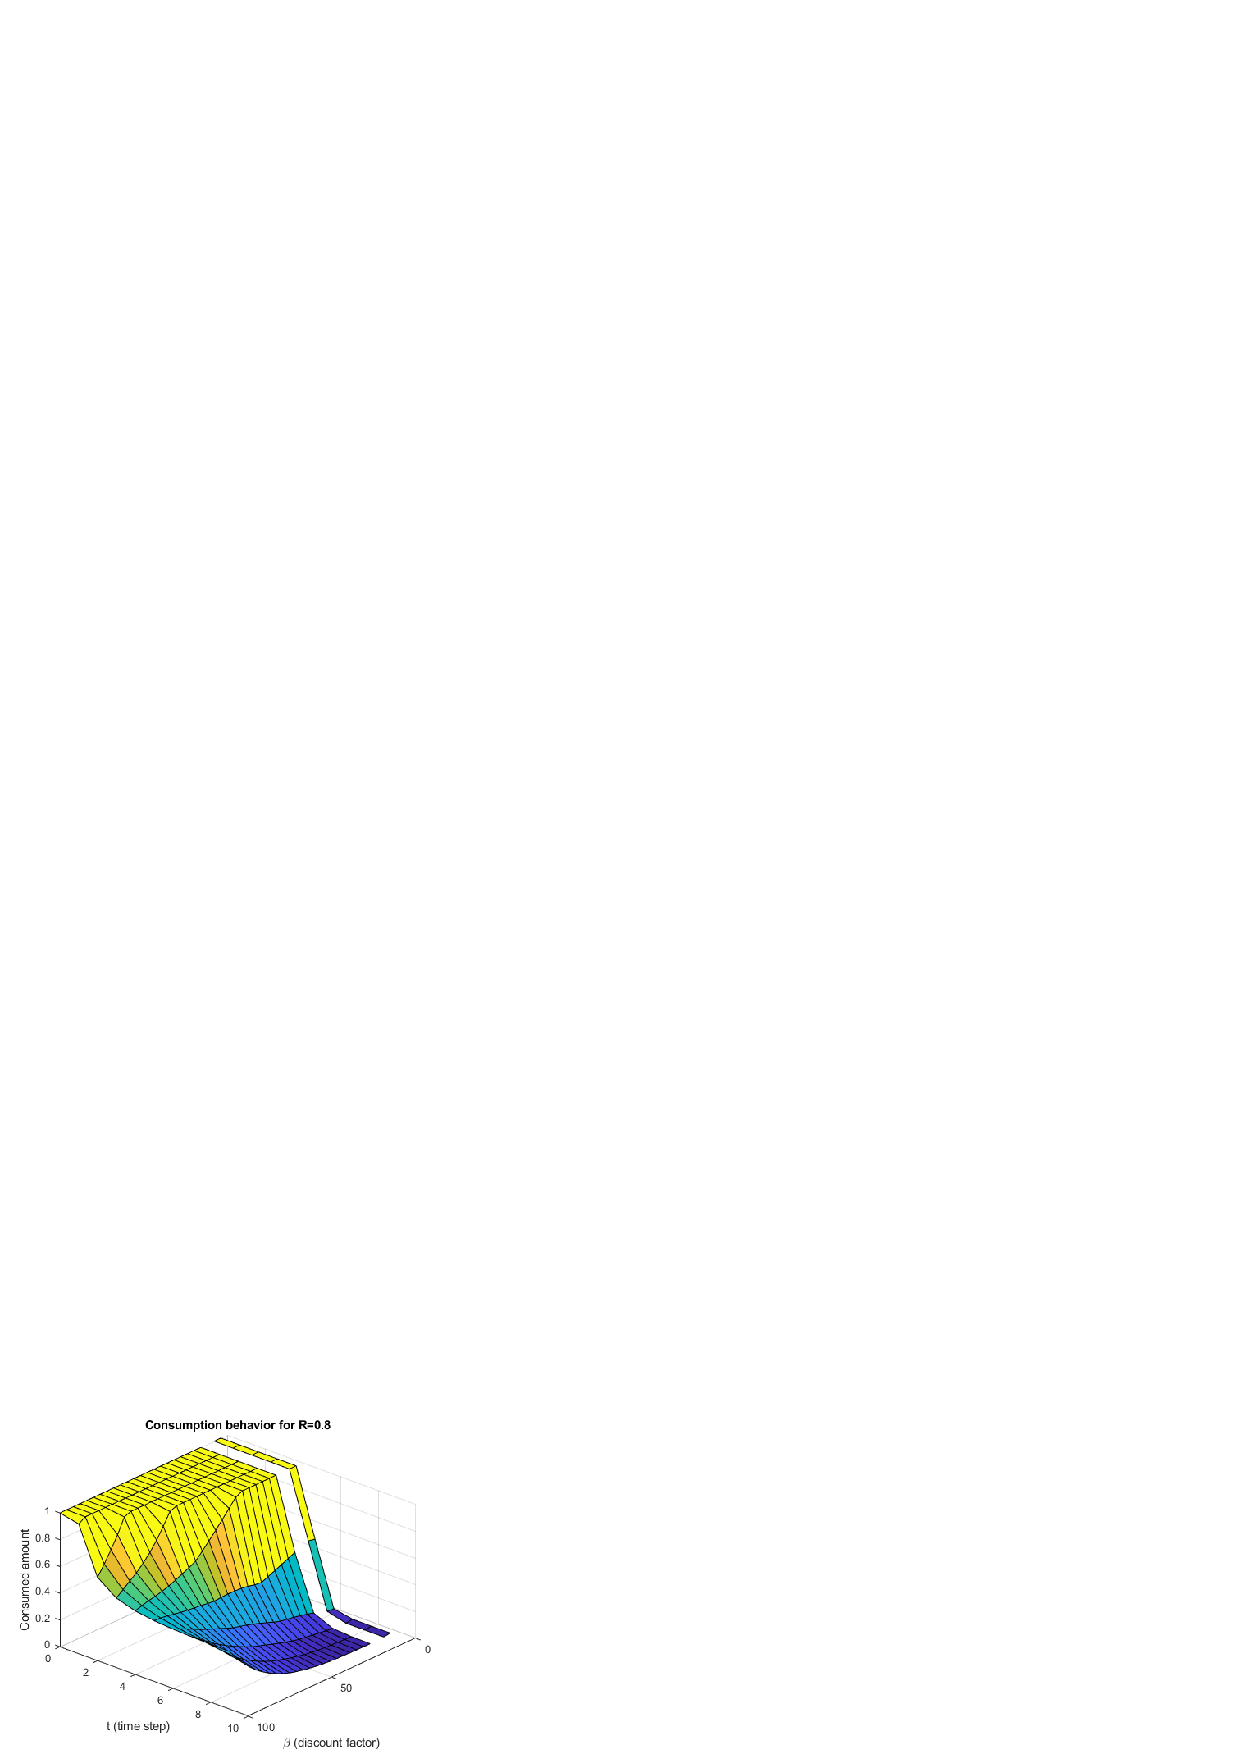
\includegraphics[width=12cm,height=8cm]{figures/r08_consumption.pdf}
\end{figure}


\begin{figure}
\caption{Optimal labor strategy for various $\beta$ and $m(1)=0.5$, R=0.8, no market clearing, Ponzi not allowed}\centering
\includegraphics[width=12cm,height=8cm]{figures/r08_labor.pdf}
\end{figure}


As it can be seen (on graphs following this page), for low $\beta$, the solution found is to maximize initial consumption and to minimize initial labor. The mechanism which allows this behavior is interest rate (R). As beta rises, we see that consumption begins to spread more evenly. 

Now let us analyze the dual variables and the values they attain. From those variables, we can comment on duality of the problem and also on the which constraints are active.

Again for the same R (=0.8) and same initial income (m=0.5) let us now plot the duality variables and afterwards let us comment on them.

\begin{figure}
\caption{Dual variable $\lambda$ for varying $\beta$ and $m(1)=0.5$, R=0.8, no market clearing, Ponzi not allowed}
\centering
\includegraphics[width=12cm,height=8cm]{figures/r08_lambda.pdf}
\end{figure}


\begin{figure}
\caption{Dual variable $\sigma$ for various $\beta$ and $m(1)=0.5$, R=0, no market clearing, Ponzi not allowed (errata: X axis is $\beta$ and not time!)}
\centering
\includegraphics[width=12cm,height=8cm]{figures/r08_sigma.pdf}
\end{figure}


\begin{figure}
\caption{Dual variable $\rho$ for various $\beta$ and $m(1)=0.5$, R=0.8, no market clearing, Ponzi not allowed}
\centering
\includegraphics[width=12cm,height=8cm]{figures/r08_rho.pdf}
\end{figure}


\begin{figure}
\caption{Dual variable $\epsilon$ for various $\beta$ and $m(1)=0.5$, R=0.8, no market clearing, Ponzi not allowed}\centering
\includegraphics[width=12cm,height=8cm]{figures/r08_epsilon.pdf}
\end{figure}

Important results can be obtained from these graphs of dual variables. Let us first denote which dual variable corresponds to which constraint and at the same time discuss the graphs obtained:

\begin{itemize}
\item $\epsilon: 0\leq c \leq 1$ \\

for different $\beta$s, this variable is always 0. This means that for high interest rates, we are always inside this boundary and never at the boundary. Only for very low  beta values, we begin to come at $0\leq c$ boundary, since with bonds the consumer chooses to spend early and work afterwards to compensate. This dual variable symbolizes how "unworthy" is a consumption good. 

\item $\rho: 0\leq l \leq 1$ \\

for different $\beta$s, this variable is very high at initial times then gets low. This means that the incentive is to work less when it matters for the utility, afterwards it becomes zero. This dual variable symbolizes how "worthy" is leisure, (i.e. a shadow price) 

\item $\lambda: m(t+1) + s(t+1) = m(t) + (1+R)s(t) + p(k)c(k) + tau(k) - p(k)c(k)$\\

this variable decreases with time and increases with beta. It is not wrong to consider this one as an incentive to "print money". The reason is, lambda is the dual variable weighing the constraint of "earned money is equal to spent money". As this dual variable gets away from zero, we see that the consumer is in demand of more money but is not able to get since he did not work hard enough.

\item $\sigma: s(N-1)=0 $\\

this variable increases with beta. This constraint was on "to leave debt for the offsprings". It makes sense since as the beta increases, the consumption at later life stages begins to be important for the individual, hence the incentive to "keep the spending trend as is." So $\sigma$ is the incentive of "leaving debt to offsprings".

\end{itemize}
\printbibliography
\newpage
%\printbibliography[heading=bibintoc]
%\label{bib:mybiblio}
\appendix
\section*{CVX MATLAB Code}\label{ch:appAlabel}
Below is given the CVX code for this problem.
%\lstinputlisting{bib/umax.m}

\end{document}